\documentclass[a4paper,12pt]{article}
\usepackage[utf8]{inputenc}
\usepackage{graphicx}
\usepackage{geometry}

\usepackage{setspace}
\usepackage{parskip}

\begin{document}

\begin{titlepage}
    \centering
    \begin{flushright}
        
\includegraphics[width=0.5\textwidth]{images/HFU-Logo.png}
    \end{flushright}
    
    \vspace{4cm}
    
    {\Large \textbf{Dokumentation}}\\[0.5cm]
    {\huge \textbf{Digitale Influencer}}\\[1.5cm]
    
    \textbf{Semesterprojekt Sommersemester 2025}
    
    \vfill
    
    \begin{flushleft}
    \textbf{Referent:} \\
    Herr Prof. Dr. Pascal Laube\\[2.5cm]
    
    \textbf{Autoren:} \\
    Marvin Jonas Kern \\
    Kevin Maisler \\
    Julia Maria Riebel \\
    Bünyamin Sener \\
    \end{flushleft}
    
    \vfill
    \begin{center}
        {\large \today}
    \end{center}
\end{titlepage}

\renewcommand*\contentsname{Inhaltsverzeichnis}
\tableofcontents
\newpage

\section{Einleitung}
Im Sommersemester 2025 wurde im Rahmen der Studiengänge Angewandte Informatik und IT-Produktmanagement an der Hochschule Furtwangen ein Projekt mit dem Titel „Digitale Influencer – Aufbau einer virtuellen Social Media Präsenz“ durchgeführt. Unter der Betreuung von Prof. Dr. Pascal Laube arbeitete ein vierköpfiges Studierendenteam daran, innerhalb eines Semesters eine vollständig digitale Influencer-Persona zu konzipieren, technisch umzusetzen und auf relevanten sozialen Netzwerken sichtbar zu machen und zu etablieren. \\\\
Ziel dieses Projekts war es, mithilfe moderner KI-Tools eine virtuelle InfluencerIn zu erschaffen, die durch automatisiert erstellte Foto- und Videoinhalte eine möglichst große Reichweite und Followerzahl generieren kann. Dabei lag der Fokus insbesondere auf der Entwicklung einer einzigartigen digitalen Identität, der strategischen Content-Planung sowie der algorithmischen Optimierung der Inhalte und Interaktionen auf Plattformen wie Instagram und TikTok.\\\\
Die Projektarbeit umfasste neben der technischen Umsetzung auch kreative und analytische Aufgaben: von der Recherche aktueller Social-Media-Trends über die KI-basierte Content-Produktion bis hin zur kontinuierlichen Auswertung von \\ Engagement-Daten zur Strategieoptimierung. Die Herausforderung bestand darin, technologische Innovation mit kreativem Storytelling zu verbinden – eine interdisziplinäre Aufgabe, die ein hohes Maß an Teamarbeit, Experimentierfreude und digitale Affinität erforderte.

\newpage

\section{Vorbereitungen}

In diesem Kapitel werden die allgemeinen Vorbereitungen für dieses Projekt behandelt. 

\subsection{Rechtliche Ausgangslage}

\subsection{Marktanalyse}

Die Entwicklung eines digitalen Influencers erfordert ein fundiertes Verständnis der aktuellen Markt- und Zielgruppenlage. In diesem Zusammenhang wurden sowohl bestehende Trends im Bereich virtueller Persönlichkeiten als auch konkrete Plattformdaten analysiert, um die strategische Ausrichtung des Projekts zu begründen. 

\textbf{Aktuelle Trends und Relevanz} \\
Virtuelle Influencer sind in den letzten Jahren zunehmend in den Fokus von Marken, Plattformen und Nutzer:innen gerückt. Digitale Persönlichkeiten wie Lil Miquela, Lu do Magalu oder Aitana Lopez  erzielen auf Social Media Reichweiten und Interaktionen ganz ohne physische Existenz. Parallel dazu steigt das gesellschaftliche Interesse an Themen wie Persönlichkeits- entwicklung, Coaching und Mental Health. \\\\
Besonders auffällig ist, dass die Akzeptanz gegenüber KI-gestützten Inhalten bei der Generation Z und den Millennials stetig wächst. Diese Gruppen zeigen sich offen für neue Formate, experimentelle digitale Erlebnisse und alternative Identifikationsfiguren. Dies sind  ideale Voraussetzungen für das Konzept eines KI-basierten Influencers mit beratendem, sowie motivierendem Charakter. 

\textbf{Wettbewerbsanalyse} \\
Eine gezielte Wettbewerbsanalyse zeigte, dass es im Bereich der inspirierenden, mentorartigen virtuellen Influencerderzeit nur wenig direkte Konkurrenz gibt. Während es viele menschliche Influencer mit Coaching-Charakter gibt, wie etwa Ali Abdaal oder Mel Robbins, ist das Feld der virtuellen Mentoren bislang kaum besetzt. Daraus ergibt sich eine vielversprechende Nische mit Differenzierungspotenzial. \\

\textbf{Zielgruppenanalyse} \\
Basierend auf Plattformdaten und thematischer Ausrichtung wurde folgende Zielgruppe definiert:
\begin{itemize}
    \item Alter: 16–35 Jahre
    \item Geschlecht: alle
    \item Bildung: Schüler:innen, Studierende, Berufseinsteiger:innen
    \item Bedürfnisse: Motivation, Struktur, Inspiration, Karriereorientierung
    \item Werte: Offenheit, Selbstreflexion, digitale Affinität
    \item Pain Points: Überforderung, Prokrastination, mangelnde Orientierung
    \item Verhalten: tägliche Nutzung sozialer Medien, bevorzugt kurze, motivierende Inhalte (z.B. Reels oder Zitat-Posts), aktive Beteiligung durch Likes, Kommentare und Story-Interaktionen \\
\end{itemize} 

\textbf{Plattformwahl} \\
Die Wahl der Plattform fiel auf Instagram, da sie optimal zur Zielgruppe passt. Mit über 30 Millionen Nutzer:innen allein in Deutschland und einem Hauptanteil von 62,3\% zwischen 18 und 34 Jahren ist die Plattform eine zentrale Plattform für die ausgewählte Zielgruppe .
Übersicht der Vorteile, die Instagram bietet:
\begin{itemize}
    \item Visuelle Ausrichtung: ideal für den ästhetisch gestalteten Content eines virtuellen Influencers
    \item Vielfalt an Formaten: Reels, Karussell-Posts, Storys, Highlights
    \item Hohe Interaktionsmöglichkeiten: durch Sticker, Umfragen, DMs
    \item Algorithmische Reichweite: insbesondere für neue Accounts mit relevantem Content
\end{itemize}
Zudem lassen sich durch gezielte Hashtag-Strategien, Posting-Zeiten sowie ein einheitliches visuelles Design mit klaren Botschaften starke Wiedererkennungswerte schaffen.


\subsection{Toolrecherche}

Um die Anforderungen unseres Projekts, insbesondere die vollautomatisierte Generierung realistischer Bildinhalte für eine digitale Influencer-Persona bestmöglich umzusetzen, wurde eine umfassende Recherche und Analyse geeigneter Softwaretools durchgeführt. Der Fokus lag dabei auf folgenden Auswahlkriterien:
\begin{itemize}
    \item Realistische Bildqualität
    \item Automatisierbarkeit über eine API (z.B. mit Python)
    \item Kostenfreiheit
    \item Open-Source-Verfügbarkeit
    \item Konsistente Bildausgabe für ein gleichbleibendes Gesicht
\end{itemize}

Im Folgenden werden die untersuchten Tools vorgestellt. \\

\subsubsection{Bildgenerierung} \\

\textbf{ChatGPT (mit DALL·E)} \\
ChatGPT in der kostenpflichtigen Version „ChatGPT Plus“ bietet integrierten Zugriff auf das KI-Bildgenerierungstool DALL·E. Die erzeugten Bilder sind qualitativ hochwertig, und Funktionen wie Inpainting sind bereits implementiert.
Einschränkend ist jedoch die fehlende API-Zugänglichkeit für Bildgenerierung: DALL·E kann derzeit nur direkt in der ChatGPT-Oberfläche verwendet werden. Eine automatisierte Ansteuerung über Python ist nicht möglich. Zudem ist für den Zugriff eine kostenpflichtige Lizenz erforderlich.
\\

\textbf{Stability AI (Stable Diffusion API)} \\
Stability AI stellt mit Stable Diffusion ein leistungsfähiges Bildgenerierungsmodell bereit. Es kann über eine offizielle API angesteuert werden, was prinzipiell eine automatisierte Integration in Workflows ermöglicht.
Allerdings basiert das Nutzungsmodell auf einem Credit-System, bei dem jede Bildgenerierung mit Kosten verbunden ist. Dadurch ist der Einsatz für eine regelmäßige, automatisierte Bildproduktion potenziell mit höheren Betriebskosten verbunden.

\begin{figure}[h]
    \centering
    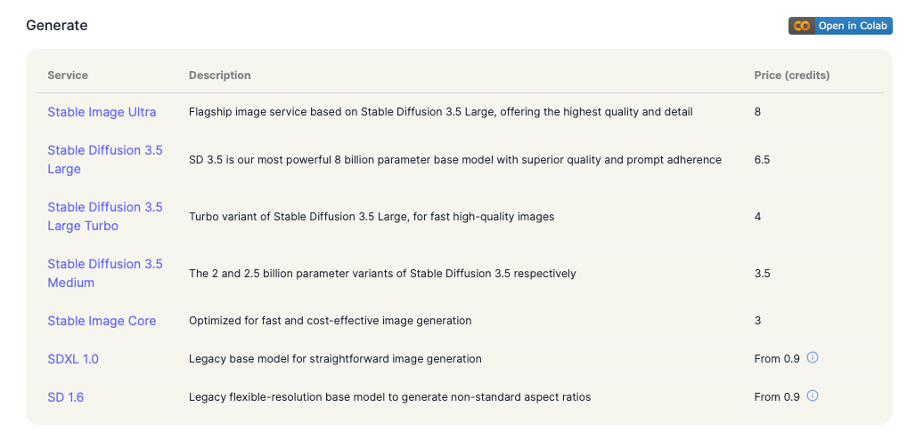
\includegraphics[width=0.8\textwidth]{images/StabilityAI.png}
    \caption{Tabellarische Darstellung der Nutzungskosten von Stability AI für Bildgenerierungen}
    \label{fig:stabilityai}
\end{figure}


\textbf{Hugging Face} \\
Hugging Face bietet eine Plattform mit zahlreichen KI-Modellen, darunter viele Varianten von Stable Diffusion, DreamBooth und ControlNet. Besonders hervorzuheben ist die API-Integration, über die sich Bildgenerierung auch automatisiert per Python-Skript anstoßen lässt.
Viele Modelle auf Hugging Face sind kostenfrei nutzbar, wobei es je nach Nutzungslast Einschränkungen hinsichtlich Rechenleistung und Geschwindigkeit geben kann.
\\

\textbf{Fooocus} \\
Fooocus ist ein Open-Source-Tool zur KI-Bildgenerierung auf Basis von Stable Diffusion. Es zeichnet sich durch eine besonders benutzerfreundliche Oberfläche aus, die komplexe Parameter automatisch im Hintergrund konfiguriert. Die Bildgenerierung erfolgt ausschließlich über Text-Prompts, was die Bedienung stark vereinfacht.
Darüber hinaus bietet Fooocus Unterstützung für moderne Bildverarbeitungstechnologien wie ControlNet, Inpainting und Upscaling. Die Software kann lokal installiert und betrieben werden, was eine Nutzung ohne laufende Kosten und ohne externe Cloud-Dienste ermöglicht.
\\

\subsubsection{Textgenerierung}

\textbf{Ollama} \\
Ollama ist eine Laufzeitumgebung für lokale Large Language Models (LLMs), mit der sich Modelle wie LLaMA 3, Mistral oder Zephyr effizient auf dem eigenen System ausführen lassen. Das Tool bietet eine einfache CLI-Schnittstelle und ist speziell für lokale Automatisierungsszenarien konzipiert. Besonders positiv hervorzuheben ist die Möglichkeit, auf Open-Source-Modelle zuzugreifen, die lokal laufen und keine Verbindung zu externen Cloud-Diensten erfordern.
\\

\textbf{OpenAI GPT (Playground / API)} \\
Das GPT-Modell von OpenAI wurde im Rahmen der Recherche aufgrund seiner hervorragenden Textqualität und vielfältigen Anwendungsmöglichkeiten betrachtet. Jedoch setzt die Nutzung eine kostenpflichtige Lizenz sowie den Zugriff über eine API voraus, was den datenschutzfreundlichen und lokalen Betrieb erschwert. Zudem ist der direkte Zugriff über die Benutzeroberfläche (Playground) nicht automatisierbar.
\\

\textbf{Hugging Face Transformers} \\
Hugging Face bietet eine große Auswahl an vortrainierten Sprachmodellen, die entweder lokal oder über Cloud-Dienste betrieben werden können. Die Plattform ist offen und gut dokumentiert, allerdings sind viele der Modelle im Vergleich zu aktuellen LLMs wie GPT-4 oder LLaMA 3 weniger leistungsfähig. Die Einrichtung erfordert zudem technisches Vorwissen und zusätzliche Infrastruktur.
\\

\textbf{Google Gemini (ehemals Bard)} \\
Google Gemini ist ein KI-gestützter Textgenerator, der über eine benutzerfreundliche Oberfläche im Browser zugänglich ist. Die erzeugten Texte sind kreativ und sprachlich variabel. Da jedoch keine API-Zugänglichkeit vorhanden ist und die Nutzung ausschließlich manuell erfolgen kann, eignet sich das Tool nicht für automatisierte Prozesse.

\clearpage

\section{Auswahl der Technologien}
\subsection{Python}

Python wurde im Projekt als zentrale Programmiersprache eingesetzt und bildete die technische Grundlage für nahezu alle automatisierten Prozesse. Die Sprache eignet sich besonders gut für die Kombination aus künstlicher Intelligenz, Web-APIs und Automatisierungslogik – drei Kernbereiche, die das Projekt vereinte. Die klare Syntax, die starke Community und die riesige Auswahl an verfügbaren Bibliotheken machen Python zu einem bevorzugten Werkzeug für schnelle Entwicklung und zuverlässige Integration.

Im Projektkontext wurde Python genutzt, um Bild- und Textgenerierungsprozesse zu steuern, lokale KI-Modelle anzusprechen (z.\,B. über die Kommandozeile mit Ollama), Bilddateien zu verwalten, sowie automatisierte Inhalte an Instagram zu übermitteln. Dafür kamen unter anderem Bibliotheken wie \texttt{subprocess} (zur Systemansteuerung), \texttt{os} (Dateioperationen), \texttt{requests} (API-Kommunikation), \texttt{json} (Datenstrukturierung) und \texttt{schedule} (Task-Planung) zum Einsatz.

Ein entscheidender Vorteil lag in der nahtlosen Integration mit GitHub Actions, wodurch sich Python-Skripte zeit- oder ereignisbasiert auf einem Server ausführen ließen – ganz ohne manuelles Eingreifen. So konnten beispielsweise neue Inhalte vollautomatisch generiert und veröffentlicht werden, sobald ein geplanter Posting-Zeitpunkt erreicht war.

Auch komplexere Prozesse wie die Auswahl passender Hashtags, das Einbinden von Variablen in Texttemplates oder der Umgang mit unterschiedlichen Inhaltsformaten ließen sich in Python übersichtlich und modular abbilden. Python ermöglichte es dem Team, technische Flexibilität mit klarer Wartbarkeit zu verbinden – ein wesentlicher Erfolgsfaktor im Hinblick auf die Skalierbarkeit und Wiederverwendbarkeit des Projektcodes.

\subsection{Github}

GitHub diente im Projekt nicht nur als zentrales Versionsverwaltungssystem, sondern spielte auch eine tragende Rolle in der automatisierten Ausführung der technischen Abläufe. Über die Plattform wurde der gesamte Quellcode entwickelt, dokumentiert und versioniert. GitHub ermöglichte es dem Team, effizient verteilt zu arbeiten, Änderungen nachzuvollziehen und reproduzierbare Ergebnisse zu sichern.

Besonders zentral war der Einsatz von GitHub Actions. Damit konnten Workflows definiert werden, die auf bestimmte Ereignisse reagieren – etwa das Hinzufügen neuer Bilddateien, geplante Zeitpunkte oder manuelle Trigger. Die automatisierte Generierung und Veröffentlichung von Social-Media-Inhalten basierte auf diesen Workflows. So wurde unter anderem bei jedem neuen Bild automatisch ein Python-Skript ausgeführt, das sowohl Text generierte (via Ollama) als auch Bild und Beschreibung über die Meta Graph API an Instagram übermittelte.

Für den sicheren Umgang mit sensiblen Informationen wie API-Zugängen oder Tokens wurden die GitHub Secrets genutzt. Sie ermöglichten es, vertrauliche Daten wie Zugriffstoken für die Meta-Plattform oder interne Variablen sicher im Repository zu hinterlegen, ohne dass diese im Quellcode sichtbar waren. Die Secrets wurden automatisch zur Laufzeit der Actions in das jeweilige Skript eingebunden und konnten so ohne manuelle Eingabe sicher verwendet werden.

Ein weiterer Vorteil von GitHub Actions war die einfache Wartbarkeit und Erweiterbarkeit: neue Automatisierungsschritte konnten modular ergänzt werden, etwa für Statusanzeigen, Log-Dateien oder Validierungen. Die Kombination aus Versionskontrolle, Automatisierung und sicherem Geheimnismanagement machte GitHub zu einem zentralen Baustein für die technische Struktur und Effizienz des Projekts.

\subsection{Ollama}

Ollama wurde im Projekt als Laufzeitumgebung für lokal ausgeführte Large Language Models (LLMs) eingesetzt und bildete das Kernstück der automatisierten Textgenerierung. Das Tool ermöglicht es, moderne Sprachmodelle wie LLaMA~3, Mistral oder Zephyr direkt auf dem eigenen System zu betreiben – ohne Abhängigkeit von externen Cloud-Diensten. Diese Eigenschaft war ein zentraler Entscheidungsfaktor im Hinblick auf Datenschutz, Automatisierbarkeit und Unabhängigkeit.

Durch die schlanke Kommandozeilen-Schnittstelle ließ sich Ollama problemlos in Python-Skripte einbinden und konnte so im Rahmen automatisierter Workflows verwendet werden. Das Tool eignete sich besonders für die Generierung von Social-Media-Captions, Hashtag-Blöcken und Beschreibungstexten, da es auf vorgefertigte Prompts reagieren und konsistente Ergebnisse liefern konnte. Die generierten Texte wurden anschließend automatisch weiterverarbeitet und in die Post-Logik integriert.

Ein zusätzlicher Vorteil lag in der lokalen Kontrolle über das Modellverhalten und den Prompt-Flow: Experimentelle Anpassungen konnten sofort umgesetzt werden, ohne dass externe Abhängigkeiten berücksichtigt werden mussten. Zudem war die Nutzung von Ollama vollständig kostenlos und auch auf leistungsschwächerer Hardware praktikabel.

Im Gesamtprojekt spielte Ollama damit eine Schlüsselrolle in der textuellen Content-Produktion – effizient, lokal ausführbar und vollständig automatisierbar.

\subsection{Fooocus}

Nach der Analyse verschiedener KI-gestützter Bildgenerierungstools fiel die finale Wahl auf Fooocus. Das Open-Source-Tool erfüllte sämtliche Anforderungen unseres Projekts in Bezug auf Bildqualität, Konsistenz, Kostenfreiheit, Automatisierbarkeit und lokale Nutzbarkeit.
Fooocus basiert auf dem Modell Stable Diffusion und verfolgt einen benutzerfreundlichen Ansatz. Statt komplexer technischer Einstellungen konzentriert sich die Nutzung auf die Eingabe eines Prompts, also einer textuellen Beschreibung des gewünschten Bildinhalts. Alle weiteren Parameter wie Stil, Sampler, Bildgröße oder Upscaling werden im Hintergrund automatisch optimiert. Dies erleichtert nicht nur den Einstieg, sondern ermöglicht auch eine schnelle und konsistente Generierung hochwertiger Bilder. \\\\
Ein besonderer Vorteil von Fooocus im Kontext unseres Projekts ist die Fähigkeit, stilistisch einheitliche und visuell konsistente Bildserien zu erzeugen. Für die digitale Persona war es entscheidend, dass das Gesicht über viele Beiträge hinweg wiedererkennbar bleibt. Fooocus unterstützt hierfür moderne Technologien wie ControlNet, Inpainting und VAE-Optimierungen, mit denen sich gezielt Details im Bild verändern lassen, ohne das Gesamtbild zu verfälschen.
Durch die Open-Source-Lizenz bietet Fooocus volle Kontrolle über die Software sowie eine lokale Ausführbarkeit ohne laufende Kosten. Dies ermöglichte eine flexible Integration in bestehende Workflows und bildete eine solide Grundlage für die spätere Automatisierung des Bildgenerierungsprozesses.

\subsection{Meta-API}


\section{KI Influencer}

Im Rahmen unseres KI-Influencer-Projekts fiel die Entscheidung bewusst auf die Konzeption eines digitalen Mentors, der sich durch Tiefe, Klarheit und eine inspirierende Ausstrahlung von der Masse abheben soll. Während viele virtuelle Influencer stark auf Ästhetik oder Mode fokussiert sind, war es unser Ziel, eine Figur mit inhaltlicher Tiefe und echtem Mehrwert zu schaffen – einen Charakter, der wie ein mentaler Coach oder Berater in digitalen Zeiten agiert.

So entstand \textbf{Elias Lev}, ein KI-generierter Influencer im Alter von 31 Jahren. Sein Auftreten ist geprägt von einem \textit{urban-clean Look}, einer ruhigen, leicht stoischen Ausstrahlung und einer tech-affinen Note. Seine Sprache ist klar, direkt und inspirierend – ohne in Motivationsfloskeln zu verfallen. Elias soll vor allem Menschen zwischen \textbf{20 und 35 Jahren} ansprechen, die sich für \textit{Selbstoptimierung, mentale Klarheit, emotionale Intelligenz und die Zukunft von KI im Alltag} interessieren.

Die Inhalte, die Elias teilt, orientieren sich an etablierten Social-Media-Formaten und verbinden sie mit einem reflektierten Ton:

\begin{itemize}
    \item \textbf{Mindset Monday}: Kurze Reels mit Zitaten und Voiceover, die zum Wochenstart Denkanstöße geben
    \item Antworten auf Community-Kommentare in einem ruhigen, erklärenden Stil
    \item Beiträge zu Routinen, Umgang mit Druck und bewusster Lebensgestaltung
\end{itemize}

Sein Erscheinungsbild ist bewusst \textit{strukturiert und leicht distanziert}, um den Eindruck eines Thought-Leaders zu unterstützen – jemand, der weniger „Freund“, sondern vielmehr ein ruhiger Gegenpol zum hektischen Informationsrauschen digitaler Plattformen ist.

Um Elias visuell zu erschaffen, haben wir mithilfe von \textbf{Fooocus} ein erstes Bild generiert. Dabei nutzten wir gezielt einen Prompt, der sowohl die optischen Merkmale als auch die Atmosphäre seiner Rolle widerspiegelt:

\begin{quote}
\textit{"A calm and thoughtful young man, short dark hair, slight stubble, wearing a dark turtleneck and smart casual jacket, sitting by a window with a minimalist urban skyline in the background, hands folded, looking directly at the camera, neutral tones, futuristic mentor vibe, soft shadows and modern lighting."}
\end{quote}

Dieses Bild diente als Grundlage für die erste visuelle Iteration von Elias und spiegelt seine Funktion als \textbf{zukünftiger Mentor in einer KI-geprägten Welt} wider.


\section{Automatisierung}
\subsection{Zitatgenerierung}
Im Rahmen des Projekts spielte die automatisierte Textgenerierung eine zentrale Rolle, da sämtliche Captions für Instagram-Posts dynamisch erstellt werden sollten. Ziel war es, vollautomatisch inspirierende Lebenszitate zu generieren, diese mit passenden Schlagwörtern zu versehen und strukturiert für die spätere Verarbeitung bereitzustellen. Dies erfolgte vollständig lokal und ohne Nutzung externer Cloud-Dienste, wodurch sowohl Datenschutzaspekte als auch technische Kontrolle gewährleistet waren.

\paragraph{Eingesetzte Technologie: Ollama + LLaMA~3}

Für die Textgenerierung kam das Tool \textbf{Ollama} zum Einsatz. Es ermöglicht das Ausführen großer Sprachmodelle (LLMs) lokal auf dem eigenen System. Im Projekt wurde dabei konkret das Modell \textbf{LLaMA~3} verwendet. Die Kommunikation mit dem Modell erfolgte über eine HTTP-API, die von Ollama bereitgestellt wird.

\paragraph{Ablauf der Textgenerierung}

Das zentrale Skript \("\)generate\_content.py\("\) steuert die gesamte Generierung. Es arbeitet in mehreren Phasen:

\begin{enumerate}
    \item \textbf{Initialer Prompt:} Ein speziell formulierter Prompt wird an das Modell gesendet, um ein tiefgründiges deutsches Lebenszitat zu erzeugen, ergänzt durch 1–3 Schlagwörter. Dabei wird das Modell zur Ausgabe in einem klaren Format aufgefordert:

    \textit{Zitat (Zeilenumbruch) Stichwort1, Stichwort2, Stichwort3}

    \item \textbf{Verfeinerung in mehreren Stufen:} Die erhaltene Rohantwort wird anschließend in zwei weiteren Schritten stilistisch überarbeitet und formal bereinigt. Jeder Schritt nutzt erneut das LLM zur Umformulierung bei kontrollierter Temperatur.

    \item \textbf{Strukturierung und Speicherung:} Nach der finalen Verarbeitung wird das Zitat samt Schlagwörtern in der Datei \textit{zitate.csv} gespeichert. Die Datei enthält eine fortlaufende Nummerierung zur eindeutigen Identifikation der Einträge. Der Aufbau folgt dem Schema:

    \textit{nr,zitat,schlagworte} \\
    \textit{001,Manchmal beginnt ein neuer Weg mit einem einzigen Gedanken.,Neuanfang, Entscheidung, Perspektive}
\end{enumerate}

\subsection{Bildgenerierung}
\subsection{Automatisches Posten}

Nach der automatisierten Erstellung von Zitaten war das automatische Veröffentlichen dieser Inhalte auf Instagram ein zentraler Bestandteil des Gesamtworkflows. Ziel war es, den Postingprozess vollständig zu automatisieren – vom Laden des Bildes über das Einbetten des Zitats bis hin zur Veröffentlichung via Meta Graph API. Dies wurde durch das Python-Skript \texttt{auto\_post.py} realisiert.

\paragraph{Gesamtablauf}

Das Skript übernimmt mehrere Schritte in fest definierter Reihenfolge:

\begin{enumerate}
    \item \textbf{Bildauswahl:} Aus einem definierten Ordner (\texttt{images\_to\_post}) wird automatisch das erste verfügbare Bild (nach Dateinamen sortiert) ausgewählt.

    \item \textbf{Laden von Zitat und Schlagwörtern:} Passend zum Bildnamen (z.\,B. \texttt{003.jpg}) wird in der Datei \texttt{zitate.csv} das entsprechende Zitat samt Schlagwörtern geladen.

    \item \textbf{Gestaltung des Bildes:} Das Zitat wird typografisch auf dem Bild platziert, inklusive halbtransparenter Textbox zur besseren Lesbarkeit. Die Textzeilen werden dabei automatisch umgebrochen, zentriert und optisch ansprechend dargestellt. Die fertige Version wird als \texttt{bild\_caption.jpg} gespeichert.

    \item \textbf{Git-Commit für RAW-URL:} Da die Instagram Graph API eine öffentliche URL für das Bild benötigt, wird das neue Bild automatisch in das GitHub-Repository gepusht, um über \texttt{raw.githubusercontent.com} verfügbar zu sein.

    \item \textbf{Erzeugung der Caption:} Die Caption besteht aus dem Zitat selbst sowie einer Hashtag-Zeile. Die verwendeten Schlagwörter werden zu Hashtags umgewandelt und mit einem vordefinierten Hashtag-Block ergänzt.

    \item \textbf{Posten via Meta Graph API:} Die Bild-URL und Caption werden an die Meta-API übermittelt. Der Upload erfolgt in zwei Schritten:
    \begin{itemize}
        \item Container-Erstellung mit Bild und Text
        \item Veröffentlichung über die erhaltene Container-ID
    \end{itemize}

    \item \textbf{Archivierung:} Nach erfolgreichem Upload wird das gepostete Bild in einen Archivordner (\texttt{archive\_images}) verschoben, um doppelte Veröffentlichungen zu vermeiden.
\end{enumerate}

\paragraph{Sicherheit und API-Zugang}

Der Zugriff auf Instagram erfolgt über die offizielle \textbf{Meta Graph API} unter Verwendung eines langfristigen Zugriffstokens (\texttt{IG\_ELIAS\_PAGE\_TOKEN}). Dieser Token sowie die Nutzer-ID werden sicher in GitHub Secrets hinterlegt und über Umgebungsvariablen abgerufen.

\paragraph{Vorteile des Systems}

\begin{itemize}
    \item \textbf{Vollständige Automatisierung} ohne manuelle Eingriffe
    \item \textbf{Zuverlässige Zuordnung} von Bildern und Zitaten über Dateinummern
    \item \textbf{Datensicherheit} durch GitHub Secrets
    \item \textbf{Öffentliche RAW-URL} über GitHub als elegante Lösung für API-Anforderungen
\end{itemize}

Das System bildet damit einen robusten, erweiterbaren und wartungsarmen Workflow, um Content automatisiert auf Instagram zu veröffentlichen.
\subsection{Archivierung und Rückverfolgbarkeit}

Um die Nachvollziehbarkeit und Wiederverwendbarkeit der generierten Inhalte sicherzustellen, wurde ein durchgängiger Archivierungsmechanismus implementiert. Jeder automatisch gepostete Beitrag – bestehend aus Bild, Zitat und Schlagwörtern – wird systematisch gesichert.

\begin{itemize}
    \item Die verwendeten Bilder werden nach dem erfolgreichen Upload in einen separaten Ordner namens \texttt{archive\_images} verschoben.
    \item Die zugehörigen Zitate mit Schlagwörtern werden fortlaufend in der Datei \texttt{zitate.csv} dokumentiert.
    \item Durch die fortlaufende Nummerierung können Inhalte jederzeit eindeutig zugeordnet und bei Bedarf erneut verwendet, angepasst oder analysiert werden.
\end{itemize}

Diese strukturierte Archivierung dient als Basis für eine mögliche Wiederveröffentlichung, statistische Auswertung oder Weiterverarbeitung zu einem späteren Zeitpunkt.

\subsection{Interaktion mit Community}

\section{Follower Analyse}

\section{Herausforderungen}
\subsection{Datenschutz}
\subsection{Meta-API}
\subsubsection{Meta AI – Erste Versuche mit \texttt{instagrapi}}

Zu Beginn der technischen Umsetzung bestand eine zentrale Herausforderung darin, automatisiert Inhalte auf Instagram zu veröffentlichen – insbesondere ohne sofortigen Zugriff auf die offizielle Meta Graph API. Um die grundlegende Funktionsweise des Systems zu testen und das Zusammenspiel der einzelnen Komponenten (Textgenerierung, Bildverarbeitung, Upload) frühzeitig zu erproben, wurde in der Anfangsphase des Projekts die inoffizielle Python-Bibliothek \texttt{instagrapi} eingesetzt.

Diese Community-basierte Bibliothek ermöglicht einen einfachen Zugriff auf Funktionen der Instagram-Plattform, indem sie das Verhalten der offiziellen App technisch nachahmt. Damit ließ sich das automatische Posten aus Python heraus unkompliziert realisieren – ein entscheidender Vorteil in der frühen Entwicklungsphase, in der es zunächst darum ging, die Machbarkeit des geplanten Systems zu validieren.

Tatsächlich gelang es mithilfe von \texttt{instagrapi}, erste Inhalte erfolgreich automatisiert zu posten. Jedoch wurde schnell deutlich, dass Instagram solche automatisierten Zugriffe über inoffizielle Schnittstellen erkennen kann. Bereits nach wenigen Testläufen wurde der Zugriff als „ungewöhnlich“ eingestuft – mit der Folge, dass sich das verwendete Skript bei jedem Durchlauf erneut einloggen musste. In der Praxis bedeutete das, dass bei jeder Ausführung zusätzliche Authentifizierungsschritte erforderlich waren (z.\,B. PIN-Eingabe via E-Mail), was die Automatisierung erheblich einschränkte.

Um diese Hürde zu umgehen und dennoch erste End-to-End-Tests des Systems unter möglichst realitätsnahen Bedingungen durchführen zu können, wurde eine lokale Konfigurationsdatei auf dem Entwicklerrechner erstellt und eingebunden. Darin wurden gerätespezifische Sitzungsdaten gespeichert, sodass die Anfragen für Instagram so erschienen, als würden sie weiterhin vom ursprünglich autorisierten Endgerät ausgehen. Dieses Vorgehen ermöglichte es, erste vollständige Post-Workflows auszuführen – inklusive GitHub Actions –, ohne bei jeder Ausführung neu authentifizieren zu müssen.

Trotz dieses pragmatischen Ansatzes war stets klar, dass \texttt{instagrapi} nur als temporäre Übergangslösung diente. Die Bibliothek befindet sich in einem rechtlichen Graubereich, da sie nicht offiziell von Meta unterstützt wird, und birgt potenzielle Risiken im Hinblick auf Datenschutz, Sicherheit und Systemstabilität. Sie erfüllte jedoch ihre Funktion als technisches Testinstrument, um frühzeitig das Zusammenspiel der automatisierten Komponenten zu prüfen und das weitere Vorgehen effizient zu planen.


\subsection{Videogenerierung}

Ein zentraler Bestandteil unseres Projekts war die Idee, nicht nur Bilder, sondern auch kurze Videos automatisiert zu erzeugen und in die Content-Strategie zu integrieren. Gerade auf Plattformen wie Instagram spielen bewegte Inhalte wie Reels, Storys und Shorts eine große Rolle für die Reichweite und das Engagement der Nutzer. Dementsprechend war das Ziel, mithilfe einer KI neben Bilder auch Videos zu generieren, die zur digitalen Persönlichkeit des Influencers passen. \\\\
Dabei war eine wichtige Voraussetzung des Projekts, ausschließlich Open-Source-Tools oder kostenlose APIs zu nutzen. Der gesamte Content sollte automatisiert, datenschutzkonform und möglichst unabhängig von kommerziellen Anbietern erzeugt werden. In der Praxis stellte sich jedoch schnell heraus, dass dies im Bereich der Videogenerierung kaum möglich ist.
Nach intensiver Recherche wurde deutlich, dass es derzeit keine Open-Source-Plattform gibt, die eine kostenlose API-Schnittstelle für die KI-basierte Videogenerierung anbietet. Die wenigen existierenden Lösungen, wie etwa RunwayML oder Leonardo AI– bieten zwar beeindruckende Ergebnisse, sind jedoch nur über kostenpflichtige Abonnements nutzbar. Eine direkte Anbindung an unsere eigenen Python-Skripte zur automatisierten Erstellung und Veröffentlichung wäre damit entweder technisch nicht umsetzbar. \\\\
Auch Versuche, über Umwege (z.B. durch Kombination einzelner Open-Source-Komponenten wie Stable Diffusion und Text-to-Speech) eigene Pipelines zu bauen, zeigten sich als zu aufwendig und instabil für einen produktiven Einsatz im Projektzeitraum. Besonders problematisch war dabei der enorme Rechenaufwand sowie die fehlende zeitliche Synchronisation zwischen Bild, Ton und Animation.

Da es keine passende Open-Source-Lösung zur Videogenerierung mit API-Schnittstelle gab, musste dieses Feature im Projektverlauf verworfen werden. Stattdessen konzentrierten wir uns auf die Erstellung von Bildinhalten, welche ebenfalls einen großen Einfluss auf Reichweite und Community-Aufbau hat. Trotz dieser Einschränkung konnten wir wichtige Erfahrungen im Bereich KI-Recherche, API-Integration und Tool-Auswahl sammeln.


\section{Fazit und Zukunftsaussichten}
\section{Arbeitsaufteilung}
\end{document}
